%%%%%%%%%%%%%%%%%%%%%%%%%%%%%%%%%%%%%%%%%
% Journal Article
% LaTeX Template
% Version 1.1 (25/11/12)
%
% This template has been downloaded from:
% http://www.LaTeXTemplates.com
%
% Original author:
% Frits Wenneker (http://www.howtotex.com)
%
% License:
% CC BY-NC-SA 3.0 (http://creativecommons.org/licenses/by-nc-sa/3.0/)
%
%%%%%%%%%%%%%%%%%%%%%%%%%%%%%%%%%%%%%%%%%

%----------------------------------------------------------------------------------------
%	PACKAGES AND OTHER DOCUMENT CONFIGURATIONS
%----------------------------------------------------------------------------------------

\documentclass[twoside,a4paper]{article}

\usepackage{lipsum}

\usepackage{tikz,pgf}
\usepackage{pgfplots}
\pgfplotsset{compat=1.7}

\usepackage{textcomp}
\usepackage[sc]{mathpazo} % Use the Palatino font
\usepackage[T1]{fontenc} % Use 8-bit encoding that has 256 glyphs
\linespread{1.05} % Line spacing - Palatino needs more space between lines
\usepackage{microtype} % Slightly tweak font spacing for aesthetics

\usepackage[hmarginratio=1:1,top=32mm,columnsep=20pt]{geometry} % Document margins
\usepackage{multicol} % Used for the two-column layout of the document

\usepackage[hang, small,labelfont=bf,up,textfont=it,up]{caption} % Custom captions under/above floats in tables or figures
\usepackage{booktabs} % Horizontal rules in tables
\usepackage{float} % Required for tables and figures in the multi-column environment - they need to be placed in specific locations with the [H] (e.g. \begin{table}[H])
\usepackage{hyperref} % For hyperlinks in the PDF

\usepackage{lettrine} % The lettrine is the first enlarged letter at the beginning of the text
\usepackage{paralist} % Used for the compactitem environment which makes bullet points with less space between them

\usepackage{abstract} % Allows abstract customization
\renewcommand{\abstractnamefont}{\normalfont\bfseries} % Set the "Abstract" text to bold
\renewcommand{\abstracttextfont}{\normalfont\small\itshape} % Set the abstract itself to small italic text

\usepackage{titlesec} % Allows customization of titles
\renewcommand\thesection{\Roman{section}}
\titleformat{\section}[block]{\large\scshape\centering}{\thesection.}{1em}{} % Change the look of the section titles

\usepackage{fancyhdr} % Headers and footers
\pagestyle{fancy} % All pages have headers and footers
\fancyhead{} % Blank out the default header
\fancyfoot{} % Blank out the default footer
\fancyhead[C]{Haydn King $\bullet$ Technical Milestone Report $\bullet$ December 2012} % Custom header text
\fancyfoot[RO,LE]{\thepage} % Custom footer text

%----------------------------------------------------------------------------------------
%	TITLE SECTION
%----------------------------------------------------------------------------------------

\title{\vspace{-15mm}\fontsize{24pt}{10pt}\selectfont\textbf{A Cross-Genome
Study of the Pentatricopeptide Repeat (PPR) Protein}} % Article title

\author{
\large
\textsc{Haydn King}\thanks{Supervised by: \textsc{Dr Jorge Gon\c{c}alves} 
(Dept. of Engineering), \textsc{Dr Jim Haseloff} 
(Dept. of Plant Sciences)}\\[2mm] % Your name
\normalsize Department of Engineering \\
\normalsize University of Cambridge \\ % Your institution
\normalsize hjk38@cam.ac.uk % Your email address
\vspace{-5mm}
}
\date{}

%----------------------------------------------------------------------------------------

\begin{document}

\maketitle % Insert title

\thispagestyle{fancy} % All pages have headers and footers

%----------------------------------------------------------------------------------------
%	ABSTRACT
%----------------------------------------------------------------------------------------

\begin{abstract}

\noindent A novel control mechanism found exclusively in plants is
investigated. 
In nature, pentatricopeptide repeat (PPR) proteins are expressed in the nucleus
and targeted to organelles where they influence protein translation by RNA
binding.
The PPR family is large and diverse but almost entirely restricted to plants; 
large numbers of PPRs are found in plant genomes while very few are found
elsewhere.
Each member of this family binds preferentially to a small number of RNA
sequences, either stabilising the mRNA or preventing translation depending on
the specific binding location.
It is hoped that understanding the principles governing PPR/RNA interaction would
allow novel proteins to be designed allowing precise expression control without
cross talk, both in plant organelles and in more conventional synthetic biology
settings.

\end{abstract}

%----------------------------------------------------------------------------------------
%	ARTICLE CONTENTS
%----------------------------------------------------------------------------------------

\begin{multicols}{2} % Two-column layout throughout the main article text

\section{Introduction and Motivation}

\lettrine[nindent=0em,lines=3]{S}ynthetic biology is a relatively new
engineering discipline with the goal of applying standard engineering techniques
such as standardisation, characterisation and encapsulation of function to 
biology.
Synbio aims to use these design principles to combine existing phenomena to 
build new, artificial forms of life.
The field is often confused with its spiritual predecessor, genetic 
engineering, which although similar in some respects does not design new
organisms, but tinkers with existing ones without trying to understand the
underlying principals.
For a brief introduction to those principals, see appendix~\ref{sec:mbio}.

Synbio is often referred to as programming, but with DNA instead of computer
code.
An example project which captures this idea is Tabor's bacterial edge
detector\cite{edgeDetector}.
Bacteria were programmed to produce a colourless chemical messenger in the 
absence of light and to produce a dark pigment in the presence of light and the
chemical messenger.
When a film of these bacteria is exposed to a pattern of light and dark, the
messenger diffuses out from the dark regions and into the light, where it
stimulates the production of the pigment, leading to an edge detection effect.

While this and other such simple demonstrations show some of the potential 
of synbio, they lack immediate application and are somewhat limited.
A major problem in expanding this work is the lack of targeted reporter
molecules.
In the edge-detector example, two molecular signals are produced when light is 
not present -- AHL, a cell-to-cell signalling molecule and cI, a
transcriptional repressor molecule.
Both AHL and cI are known to affect the promoter $P_{lux-\lambda}$; while AHL 
stimulates expression, cI strongly represses it.
With expression of the dark pigment being driven by $P_{lux-\lambda}$, 
both light and AHL are required to cause the pigment to be produced.

The effect of the molecules AHL and cI on $P_{lux-\lambda}$ is one of a small
but growing number of well understood control motifs.
Since reusing the same promoter/signal in the same cell is impossible due to 
cross-talk, there are simply not enough signalling modalities available to
perform more complex calculations within the cell.
Indeed, it is often the case that signalling molecules have multiple functions
within the cell such that changing the concentration of one molecule to suit
our goals may cause a seemingly unrelated area of the cell's metabolism to
malfunction with undesirable consequences.

A more applicable synbio project was the effort to produce 
artemisinin (the most effective known anti-malarial) in a cheaper and more 
scalable way.
Artemisinin is found naturally in sweet wormwood, but it is slow and expensive
to extract directly from the plant and chemical synthesis is also an expensive
and laborious process.
Synthetic biologists were able to extract the metabolic pathway responsible for
the biosynthesis of artemisinic acid (a natural precursor) and insert it into 
yeast\cite{yeast}.
Artemisinin produced in this manner has yet to be approved for sale, but it is
hoped that it should be available at some point during 2013, at a considerably
lower price than any other method of production.

The major limiting factor in this project was yield.
In order to produce a useful amount of the drug, the pathway involved had to be
up-regulated, which led to a difficult balance -- too little and very little
artemisinic acid would be produced, too high and too much of the cell's
energy would be used, causing the cells to grow slowly if at all.
As well as this, growing yeast on an industrial scale is relatively expensive.
It is desirable therefore search for host platforms which are better suited to
biosynthesis than yeast, in order to maximise the yield to cost ratio.

Chloroplasts are a major centre for biosynthesis in plants as they perform
photosynthesis to provide energy for the plant.
The result of an ancient symbiosis, up to 1000 of these primitive cells can be 
found within each plant cell, where they make an excellent target for synbio.
They are similar to previous synbio hosts, but with access to the more
sophisticated plant cell machinery and superb potential for biosynthesis.
The native enzyme RuBisCO is so abundant in the chloroplasts that it 
can be up to 50\% of overall soluble leaf protein.
Achieving anything remotely close to this figure in a project such as the
production of artemisinin would help reduce the vast number of people who die 
of this treatable disease each year (roughly 2,000 deaths a day in 2010
\cite{malaria}).

%------------------------------------------------

\section{Project Background}

Understanding how gene expression is controlled in chloroplasts is a key step
in achieving this goal.
Unlike previous synbio targets, chloroplast genes are generally expressed
constitutively (continuously) leading to constant mRNA levels rather than 
being controlled by promoter regulation\cite{Sugita1996}.

PPR proteins are a class of signalling protein found almost exclusively in
plants\cite{Small2000}. 
They are synthesised in the nucleus and sent to organelles such as the 
chloroplast where each one binds to a specific RNA sequence.
Depending on whether the protein binds to the untranslated region within the
RNA message or over the ribosome binding site, expression is either increased 
(by preventing exonucleases from destroying the mRNA) or decreased by reducing 
ribosome activity\cite{Pfalz2009}.

PPR proteins are made up of a short targeting region followed by a series of
repeating regions which form the RNA binding site.
They may also contain a tail region which can be classified as
belonging to one of 3 different categories. 
The function of the tail region is hitherto unknown\cite{Lurin2004}.

The 3D structure of the repeating domain is not known, which making it harder
to identify the regions responsible for target binding.
Statistical analysis of a large set of experimentally verified PPR/RNA pairs
has shown a strong link between the amino acids at position 6 in repeat domain
$n$ and position 1 in repeat domain $n+1$ (hitherto referred to as position 1')
and the bound nucleotide at position $n$\cite{Barkan2012}.
Weight was added to this conjecture after a PPR protein with known binding
target was mutated such as to change its binding preference in a predictable
way\cite{Barkan2012}.

Ultimately, being able to design a PPR protein to bind to an arbitrary RNA
sequence with a pre-specified affinity would be of great use to synthetic
biology.
It would both improve our knowledge of the chloroplast and give us the
necessary tools to control expression within it and provide a convenient way to
precisely control the expression of a gene without the possibility of 
cross-talk or interference.

As a first step towards this goal, the project has the following goals:
\begin{itemize}
  \item Find and predict the binding targets of PPR proteins from several plant 
    genomes and compare those which correspond to
    similar binding targets and discover which features of the protein are
    preserved
  \item Verify that PPR-style control can be performed in a bacterial setting
    such as in \textit{E. coli}, by designing and performing a simple test 
    with known PPR/RNA binding pairs
\end{itemize}


%------------------------------------------------

\section{Completed Work}

The first challenge was to discover and annotate PPR proteins within a genome.
Many genomes have PPR proteins which have been discovered and experimentally
verified, but although in these cases the location of the protein has been
marked, the location of the internal PPR motifs has not.
Locating these motifs accurately is important as it is required in order to
identify the amino acids at positions 6 and 1', and therefore predict likely
binding domains.

The method used to locate these motifs was Hidden Markov Model (HMM) search, 
using the HMMER package, a free and open-source HMM software package.
For a brief introduction to HMMs, see Appendix~\ref{sec:HMMs}.

The basic approach used is similar to \cite{Lurin2004}, where an HMM is used to
detect PPR motifs and clusters of motifs are then extracted as putative
proteins.
The models used were those available in the Pfam database; a large collection
of protein families maintained by the Sanger institute.
Four versions of the PPR model exist in Pfam, and it was found that the latest,
PPR\_3 (retrieved from \url{http://pfam.sanger.ac.uk/family/PF13812}) gave the
best accuracy when annotating a known test protein.
As in \cite{Lurin2004}, it was expected that this model would give a large
number of false positives within an entire genome as it is statistically likely
that a PPR-like sequence will occur at random within the genome.
This is unlikely to prove a problem as we are searching for a sequence of
several motifs close together within the same reading frame, which is unlikely
to occur by chance.

Extracting a protein from a HMMER search requires considerable
post-processing, as, for example, searching for a protein model within
a DNA sequence is not natively supported by HMMER.
As outlined in appendix~\ref{sec:mbio}, DNA is translated into a sequence of
amino acids by a 3:1 code -- i.e. three nucleotides of DNA produce one amino
acid in a protein.
This means that there are six possible reading frames, 3 forward and 3 reverse
which must be searched in order to search the entirety of the protein space.
This is referred to as a six-frame translation and is not handled natively by
HMMER; it is left to the user to perform.
In order to overcome these limitations, I have begun work on pyHMMER, a python
wrapper for HMMER.
pyHMMER accepts python objects as inputs and converts to HMMER's
native format, taking six-frame translations as necessary and parses HMMER's
file output, returning it as a python object.
pyHMMER is licensed under the GPL, and is available from
\url{https://github.com/haydnKing/pyHMMER}.

Having discovered PPR motifs within a genome, clusters of motifs are discovered
where:
\begin{itemize}
  \item Each motif is a certain maximum distance from another within the
    cluster
  \item Each motif is within the same reading frame
  \item None of the motifs overlap
\end{itemize}
Having discovered such clusters, the protein can be extracted by searching
upstream for an in-frame start sequence (\textsc{atg}) and a downstream stop 
sequence (one of \textsc{tag}, \textsc{taa} or \textsc{tga}).
If the distance from start to stop sequence is too large, then the protein is
discarded as a false positive.

These putative proteins are then annotated and categorised.
Large gaps in the sequence of motifs are searched for reluctant motif regions
and small gaps between the motifs are removed.
The subgroup to which the PPR protein belongs is identified using a
\textsc{jackhmmer} search of the tail sequence using consensus sequences 
from \cite{Lurin2004}.
The organelle to which the protein is targeted is also predicted, using the
targetP prediction program.

%------------------------------------------------
\section{Preliminary Results}
\label{sec:results}

The strategy outlined above has been tested using the genome of 
\textit{Arabidopsis thaliana} (chosen as it is well studied and the focus of
\cite{Lurin2004}). 
Table~\ref{tab:CHR} shows the number of PPR proteins
extracted from each chromosome compared with those already known.
These numbers correlate well, although more proteins are discovered than have
been verified, suggesting that some may be false positives.
As discussed above, this seems unlikely -- it is more plausible that several
single proteins are registering as multiple proteins.

\begin{table}[H]
  \centering
  \begin{tabular}{c|c|c}
    Chromosome & Found & Known \\
    \hline
    1 & 98 & 78 \\
    2 & 42 & 32 \\
    3 & 59 & 50 \\
    4 & 36 & 37 \\
    5 & 60 & 57 \\
    \hline
    $\Sigma$ & 295 & 254 \\
  \end{tabular}
  \caption{Number of PPR proteins found in each chromosome of 
    \textit{Arabidopsis thaliana} and the number shown in the TAIR10 genome
    release}
  \label{tab:CHR}
\end{table}

Shown in Figure~\ref{fig:ppr} is the number of PPR proteins discovered plotted
by number of repeats.
The majority of the proteins have between 3 and 10 repeats, with few having
greater than 15 repeats.
The large number of shorter proteins present a potential problem -- if we were
to predict a specific binding sequence that is 5bp in length, the probability 
of that sequence happening at random is ${1/4}^5 \approx 10^{-4}$.
The chances of this sequence happening at random in the chloroplast is quite
high, as the chloroplast is around 120,000bp in length.
This problem is made worse by the fact that we aren't searching for a specific
sequence, rather a set of sequences whose probability of having been generated
by our HMM is above a certain threshold.
We must, therefore, be wary of false positives when searching for binding 
targets for short PPR proteins.

We cannot hope to distinguish false and true positives analytically as it is
known that some PPR proteins will bind to more than one
sequence\cite{Barkan2012}.
It is conceivable, then, that short PPR proteins do have multiple binding sites
within the chloroplast genome -- this would even be desirable, as it would
allow control of several genes with only one protein.

\begin{figure}[H]
  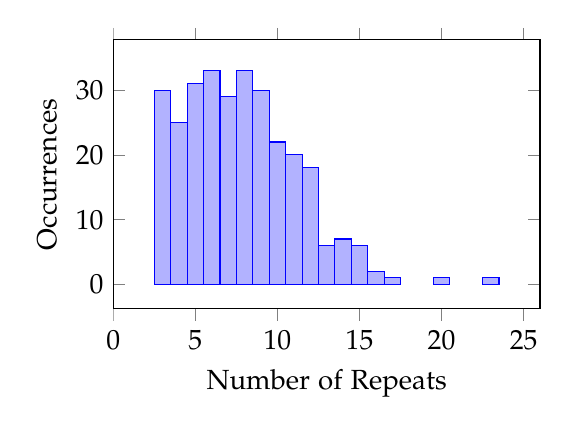
\begin{tikzpicture}
    \begin{axis}[ybar, 
      enlargelimits=0.15,
      width=7cm, height=5cm,
      xlabel={Number of Repeats},
      ylabel={Occurrences},
      bar width = 1,]
      \addplot 
      coordinates {(3,30) (4,25) (5,31) (6,33) (7,29) (8,33) (9,30) (10,22)
        (11,20) (12,18) (13,6) (14,7) (15,6) (16,2) (17,1) (20,1) (23,1)};
    \end{axis}
  \end{tikzpicture}

  \caption{Number of PPR motifs found in the PPR proteins of
    \textit{Arabidopsis thaliana}}
  \label{fig:ppr}
\end{figure}

%------------------------------------------------
\section{Further Work}

The remaining work of the project can be largely divided into three areas:
\begin{enumerate}
  \item Verify the work presented above \& account for the extra proteins
    discovered \label{todo:verify}
  \item Predict target regions within the chloroplast genome
    \label{todo:predict}
    \begin{enumerate}
      \item Build HMMs to model the target region using the statistics
        presented in \cite{Barkan2012}
      \item Search the chloroplast for potential binding sites
      \item Attempt to discover similar binding sites in closely related plants
        and perform alignments of the PPR proteins involved
      \item Use the alignments to discover the important features of the PPR
        protein which determine binding
    \end{enumerate}
  \item Verify whether PPR/mRNA based expression control is effective within
    prokaryotic bacteria such as \textit{E. coli}
    \label{todo:wet}
    \begin{enumerate}
      \item Design and build an inducible system to express a well 
        characterised PPR protein
      \item Design genes which will produce mRNA including with the PPR target
        incorporated in both positive and negative arrangements
      \item Measure the concentration of the test protein in response to
        induction (i.e. in response to the presence of the PPR)
    \end{enumerate}
\end{enumerate}

Item~\ref{todo:verify} refers to the problems discussed in 
section~\ref{sec:results} above, regarding the discovery of more PPR proteins 
than are known to exist in the genome.
This will involve careful comparison of the proteins which have been found and
those which are known to exist, and should not present much challenge.

This work is continued in item~\ref{todo:predict}, where the binding targets of
the proteins are predicted.
Building an HMM from known parameters is already implemented in pyHMMER, and
the relevant statistics are available in the literature\cite{Barkan2012}, so
this step should be trivial.
Actually discovering targets within the chloroplast is likely to present more
difficulties and is therefore not guaranteed to work; it is possible
that there might be no matches or that there are so many matches that the
prediction is meaningless.
In either scenario, the only direct way of overcoming the issue would be to
vary the model parameters, making it either more or less open to variation
depending on the specific situation.

The purpose of Item~\ref{todo:wet} is to demonstrate that PPR-based control can
be used for synthetic biology.
While understanding this phenomenon would still be useful to those studying
the chloroplast, it would have a far greater appeal if it was known to be
effective in more established synbio systems as well.
Although the test outlined is relatively simple in theory, performing this
experiment in the lab may prove to be time-consuming and difficult.
It is hoped that this will be feasible within the scope as it would clearly
contribute greatly to the value of the project.

%----------------------------------------------------------------------------------------
%	APPENDICES
%----------------------------------------------------------------------------------------

\begin{center}
  \large\textsc{Appendices}
\end{center}

\appendix

\section{Hidden Markov Models and the HMMER Package}
\label{sec:HMMs}

A Hidden Markov Model (HMM) is a statistical model of a Markov Process where
the sequence of states is unknown but a symbol is emitted from each state. 
An HMM has a set of $N$ states, 
$\Omega = \omega_{1 \ldots N}$ and an alphabet of $M$ symbols, 
$\Psi = \psi_{1 \ldots M}$. 
The probability of emitting the symbol $\psi_i$ from state $\omega_j$ is 
defined as $\theta_{\psi_i | \omega_j}$.
Similarly, the probability of transitioning from state $\omega_j$ to state
$\omega_i$ is given by $\phi_{\omega_i | \omega_j}$.
The model results in a sequence of states $x(t) \in \Omega$ which are not
observed, and a sequence of symbols $y(t) \in \Psi$ which are observed for some
range of $t$.

HMMs have proved useful in a number of fields, but have been particularly
useful in modelling biological sequences. 
In general, bioinformaticians use a special case of the HMM called a
profile-HMM or a pHMM.
A pHMM is an HMM whose network topology is fixed, as shown in.
They contain a number of nodes, each of which contains an emission state, an
insert state and a mute delete state, which either emit a single symbol, emit
one or more symbols or emit no symbols before moving to the next node
respectively.

Profile-HMMs have numerous practical advantages over general HMMs. 
Firstly, there is a significant reduction in the number of transition states
which must be calculated and stored and secondly it is possible to 
automatically
generate a pHMM from a sequence alignment using the Expectation-Maximisation
algorithm as the topology is fixed. More information is available about HMMs
and other aspects of bioinformatics in \cite{Durbin1998}.

Many of the algorithms required to build and manipulate pHMMs are implemented
in the \textsc{hmmer}\cite{HMMERguide} package, a free and open source software 
package available from \href{http://hmmer.janelia.org/}{hmmer.janelia.org}.

\section{Molecular Biology}
\label{sec:mbio}

Molecular biology is the study of the molecular basis of biology.
While the field itself is rather broad, much of it is underpinned by what is
referred to as the central dogma of molecular biology -- 
DNA makes RNA makes proteins.
This central dogma describes the flow of information within a cell and the
processes and control mechanisms which regulate this process.
Naturally, many of these processes are highly complicated and poorly
understood, but much progress has been made since the discovery of DNA in the
1950s to understand these processes.
Below is a brief introduction, aimed at the information or control engineer.

Molecules of DNA are the cell's long term storage mechanism -- recent research
estimates the half-life of DNA to be 521 years\cite{DNAhalflife}.
The first process is called \textit{transcription}, where the DNA molecule is
'read' by an RNA polymerase, producing an RNA copy of a section of the DNA.
The RNA molecule is called messenger-RNA as it is a short-lived (minutes to
hours) message.
This message is read by a ribosome, a molecule which translates the mRNA into a
protein, a process referred to as \textit{translation}.
Proteins then fold into a very specific shape determined by their 
sequence, and go on to perform many important functions within the cell.
The processes of transcription and translation are typically very tightly
controlled by the cell, as this is the main way of influencing the levels of
various proteins within the cell.

DNA consists of a sequence of four different nucleotides recorded as G,A,T and C.
When DNA is transcribed to mRNA, thymine is replaced with uracil, such that the
RNA alphabet is represented as G,A,U and C.
Proteins are a sequence of amino acids, where each acid comes from an alphabet
of 20 amino acids.
Each acid is coded for by 3 base pairs of RNA, which are referred to
collectively as a codon.
Since there are $4^3$ possible codons and only 20 amino acids, the code is
over complete -- several different codons map to the same amino acid.
As well as coding for amino acids, three special codons (UAG, UAA and UGA) are
known as stop codons as they terminate the translation of the protein.

The DNA region which codes for a protein is called a gene, and is marked by a
promoter region, to which the RNA polymerase binds at the start of
transcription.
Control is often achieved by modulating the activity of the promoter, either to
enhance or hinder the binding of RNA polymerase.
In prokaryotes, the promoter region is usually a short distance upstream from
the gene or genes to be transcribed, such that the mRNA sequence contains a
short untranslated region, followed by one or more genes and then another short
untranslated region.

Ribosomes bind to the mRNA, reading the gene and creating the appropriate
protein before detaching from the mRNA.
mRNA is more fragile than DNA but is also targeted by exonucleases, a class of
enzyme which degrade RNA molecules, preventing the production of more protein.
Similar processes exist to degrade proteins over time, recycling their amino
acids to form new proteins.
These degradation processes mean that a gene must continue to be transcribed at
a constant rate for the concentration of its protein to remain constant.


%----------------------------------------------------------------------------------------
%	REFERENCE LIST
%----------------------------------------------------------------------------------------
\tiny

\bibliographystyle{unsrt85}

\bibliography{references}

%----------------------------------------------------------------------------------------

\end{multicols}

\end{document}
